\chapter{User evaluation}
\label{chap:user-evaluation}

This chapter presents the last (and most extensive) experiment carried out in this thesis. The empirical studies exposed so far in Chapters \ref{chap:wozlearning} and \ref{chap:rllearning} essentially focused on the learning performance of rule-structured models compared to more classical representations. But albeit such experiments can provide useful insights about the model adequacy for various dialogue domains, they are not by themselves sufficient to assess the suitability of a particular modelling approach and its practical effects on the quality of the produced interactions. 

In order to corroborate our claims regarding the benefits of probabilistic rules in dialogue management and contrast them to traditional methods, we conducted an user evaluation experiment with a total of 37 users. The aim of the experiment was to compare three alternative approaches to dialogue management (two baselines and our own approach) in a human--robot interaction domain.  The three approaches respectively correspond to a purely handcrafted approach, a purely statistical approach, and a hybrid approach based on probabilistic rules. The empirical results collected through this experiment report that the  hybrid, rule-structured approach is able to outperform the two baselines on most of the metrics defined for the domain.  The metrics include not only objective metrics extracted from the interaction logs but also subjective metrics of user satisfaction, based on a survey completed by the participants after each interaction. 


The chapter is structured in three sections.  The first section describes the human-robot interaction scenario within which the experiment is carried out, and details both the state variables, system architecture, and training data made available for the domain. The second section then exposes the three alternative dialogue management approaches developed for the experiment, with a particular emphasis on the design choices that characterise each strategy.   Finally, the third section presents the user evaluation itself, and surveys the experimental setup, quality metrics, and of course the empirical results and their detailed analysis. 

\section{Interaction scenario}

The interaction scenario employed for the user evaluation is similar in most respects to the one presented in Section \ref{sec:rllearning-experiments}, modulo some minor adaptations to circumscribe more precisely the task to be performed.\footnote{This change was suggested by several participants in the previous study.} The interactions revolve around a human user and a Nao robot standing on a large table, as illustrated in Figure \ref{fig:scenario}.  The purpose of the interaction is to instruct the robot to (1) walk to the other end of the table without bumping into the imaginary walls placed in the middle of the scene, (2) pick up the designated object, (3) bring it back to the left side of the table, and (4) release it on a yellow landmark.  The robot is able to perceive the presence, colour and location of each physical object thanks to visual markings placed at their top.  It can also grasp each object with the help of permanent magnets fixed inside the hands of the robot. 

\begin{figure}[h]
\vspace{3mm}
\centering
\includegraphics[scale=0.13]{imgs/scenario.jpg} \vspace{3mm}
\caption{Interaction scenario for the experiment.  On the right side of the table stand two objects (one red and one blue).  Imaginary walls (in green) are also placed on the table, as well as a yellow landmark depicting the final destination of the robot. }
\label{fig:scenario}
\end{figure}


\subsection{Dialogue domain}

\subsubsection*{User intentions and actions}

As for the previous experiment, we represent each basic instruction (such as moving forward, turning left, picking up an object, etc.) as a distinct user intention $i_u$. After the fulfilment of each instruction, the user intention is reinitialised to represent the next instruction to perform.  The possible user intentions for the domain are shown in Table \ref{table:userintents_exp3}.  


One can observe a few changes compared to the Wizard-of-Oz study presented in Section \ref{sec:rllearning-experiments}. The basic movements are now augmented with a second argument specifying the duration of the movement, e.g.\ short or long. The human user can therefore explicitly request the robot to perform a short or long movement. A new type of movement has also been added, $\mathrm{Move(Turn)}$ to make the robot turn around by 180 degrees.  Finally, specific intentions are used to capture the opening (engagement) and closing (disengagement) phases of the dialogue. 

The possible user actions $a_u$, listed in Table \ref{table:userdas_exp3} correspond to the verbal realisations of these user intentions. The user can directly utter an instruction, ask the robot to repeat its last movement, or respond to a clarification or confirmation request.   The user action $\mathrm{Ask(Stop)}$ can also be used to command the robot to stop its current movement, while grounding actions represents explicit  feedback provided by the user on the robot behaviour.

\subsubsection*{System actions}
As shown in Table \ref{table:systemdas_exp3}, the system actions $a_m$ include: \begin{itemize}
\item Physical movements to move around in various directions and lengths, pick up or put down physical objects on the table, or stop the current move.
\item Verbal responses to describe the robot's current perception or tell the user that it cannot perform a requested movement due to some impeding factor (e.g.\ not being able to pick up an object whose location is currently unknown). 
\item Clarification and confirmation requests, such as asking the users to repeat their last utterance, or confirming a particular intention.
\end{itemize}

Instead of representing grounding actions in a separate category of actions (as in Table \ref{table:systemdas_exp2}), the grounding acts are now directly coupled to the system actions. The selection of the system action $\mathrm{Do}(x)$ therefore triggers both a grounding action (\utt{Ok, now doing $x$}) and the simultaneous execution of the corresponding physical movement. 

\renewcommand{\arraystretch}{1.3}

\begin{table}[p!]
\begin{footnotesize}
\begin{tabular}{p{60mm}} 
$\cdot$ $\mathrm{Move}(x,y) $ \\ $ \ \ \ \ \ \text{ where } x=\{\mathrm{Left,Right,Forward,}$ \\ $\ \ \ \ \ \ \ \ \ \ \ \ \ \ \ \ \ \ \ \ \ \ \ \ \ \mathrm{Backward}\} $ \\ $ \ \ \ \ \ \ \text{ and } y = \{\mathrm{Short, Long}\}$ \\
$\cdot$ $\mathrm{Move(Turn)} $ \\
$\cdot$ $\mathrm{PickUp}(x) $ \\ $\ \ \ \ \  \text{ where } x \text{ is an object identifier}$ 
\end{tabular}
\hspace{2cm}
\begin{tabular}{p{60mm}} 
$\cdot$ $\mathrm{ReleaseObject} $ \\
$\cdot$ $\mathrm{WhatDoYouSee}$ \\
$\cdot$ $\mathrm{DoYouSee}(x) $ \\ $\ \ \ \ \  \text{ where } x \text{ is an object identifier}$ \\
$\cdot$ $\mathrm{Greeting}$ \\
$\cdot$ $\mathrm{Closing}$ 
\end{tabular}
\end{footnotesize}
 \caption{List of user intentions $i_u$} 
\label{table:userintents_exp3}
\end{table}


\begin{table}[p!]
\begin{footnotesize}
\begin{tabular}{p{60mm}} 
$\cdot$ $\mathrm{Ask(Move(x,y))} $ \\ $ \ \ \ \ \ \text{ where } x=\{\mathrm{Left,Right,Forward,}$ \\ $\ \ \ \ \ \ \ \ \ \ \ \ \ \ \ \ \ \ \ \ \ \ \ \ \ \mathrm{Backward}\} $ \\ $ \ \ \ \ \ \ \text{ and } y = \{\mathrm{Short,Long}\}$ \\
$\cdot$ $\mathrm{Ask(Move(Turn))} $ \\
$\cdot$ $\mathrm{Ask(PickUp(x))} $ \\ $\ \ \ \ \  \text{ where } x \text{ is an object identifier}$ \\ $\ \ \ \ \  \text{ or }  \mathrm{Other} \text{ if the reference is not resolved}$ \\
$\cdot$ $\mathrm{Ask(ReleaseObject)} $ \\
$\cdot$ $\mathrm{RepeatLast}$ \\
$\cdot$ $\mathrm{Ask(Stop)}$ 
\end{tabular}
\hspace{2cm}
\begin{tabular}{p{60mm}} 
$\cdot$ $\mathrm{Ask(WhatDoYouSee)}$ \\
$\cdot$ $\mathrm{Ask(DoYouSee(x))} $ \\ $\ \ \ \ \  \text{ where } x \text{ is an object identifier }$ \\ $\ \ \ \ \  \text{ or }  \mathrm{Other} \text{ if the reference is not resolved}$ \\
$\cdot$ $\mathrm{Confirm}$ \\
$\cdot$ $\mathrm{Disconfirm}$ \\
$\cdot$ $\mathrm{Grounding}$ \\
$\cdot$ $\mathrm{Greet}$ \\
$\cdot$ $\mathrm{Close}$ \\
$\cdot$ $\mathrm{Other}$ 
\end{tabular}
\end{footnotesize}
 \caption{List of user actions $a_u$} 
\label{table:userdas_exp3}
\end{table}

\begin{table}[p!]
\begin{footnotesize}
\begin{tabular}{p{60mm}} 
$\cdot$ $\mathrm{Do}(x) $ \\ $ \ \ \ \text{ where } x=\{\mathrm{Move}(y,z), \mathrm{Move(Turn)},$ \\ $\ \ \ \ \ \ \ \ \ \ \ \ \ \ \ \ \ \ \ \ \ \ \ \mathrm{PickUp}(a),  \mathrm{ReleaseObject},$ \\ $\ \ \ \ \ \ \ \ \ \ \ \ \ \ \ \ \ \ \ \ \ \ \ \mathrm{Stop}\} $ \\ $ \ \ \ \ \ \ \text{ and } y = \{\mathrm{Left,Right,Forward,}$ \\ $ \ \ \ \ \ \ \ \ \ \ \ \ \ \ \ \ \ \ \ \ \ \ \ \mathrm{Backward}\} $ \\ $ \ \ \ \ \ \ \text{ and } z = \{\mathrm{Short,Long}\}$ \\ $ \ \ \ \ \ \  \text{ and } a = \ \text{an object identifier}$ \\
$\cdot$ $\mathrm{Excuse}(x) $ \\ $ \ \ \  \text{ where } x = \{\mathrm{UnseenObject}$ \\ $\ \ \ \ \ \ \ \ \ \ \ \ \ \ \ \ \ \ \ \ \ \ \ \mathrm{UnresolvedReference},$  \\ $\ \ \ \ \ \ \ \ \ \ \ \ \ \ \ \ \ \ \ \ \ \ \ \mathrm{NoCarriedObject,}$ \\ $\ \ \ \ \ \ \ \ \ \ \ \ \ \ \ \ \ \ \ \ \ \ \ \mathrm{AlreadyCarryObject}\}$ \\
$\cdot$ $\mathrm{Greet}$ \\
$\cdot$ $\mathrm{Goodbye}$ 
\end{tabular}
\hspace{2cm}
\begin{tabular}{p{60mm}} 
$\cdot$ $\mathrm{Describe}(x) $ \\ $ \ \ \  \text{ where } x = \ \text{a (possibly empty) list}$ \\ $ \ \ \ \ \ \ \ \ \ \ \ \ \ \ \ \ \ \ \ \ \ \ \  \text{of object identifiers}$ \\
$\cdot$ $\mathrm{ConfirmDetection}$ \\
$\cdot$ $\mathrm{DisconfirmDetection}$  \\
$\cdot$ $\mathrm{AskClarify}$ \\
$\cdot$ $\mathrm{AskConfirm}(x) $\\ $ \ \ \ \text{ where } x=\{\mathrm{Move}(y,z), \mathrm{Move(Turn)},$ \\ $\ \ \ \ \ \ \ \ \ \ \ \ \ \ \ \ \ \ \ \ \ \ \ \mathrm{PickUp}(a),  \mathrm{ReleaseObject},$ \\ $\ \ \ \ \ \ \ \ \ \ \ \ \ \ \ \ \ \ \ \ \ \ \ \mathrm{Stop}\} $ \\ $ \ \ \ \ \ \ \text{ and } y = \{\mathrm{Left,Right,Forward,}$ \\ $ \ \ \ \ \ \ \ \ \ \ \ \ \ \ \ \ \ \ \ \ \ \ \ \mathrm{Backward}\} $ \\ $ \ \ \ \ \ \ \text{ and } z = \{\mathrm{Short,Long}\}$ \\ $ \ \ \ \ \ \  \text{ and } a = \ \text{an object identifier}$ \end{tabular}
\end{footnotesize}
 \caption{List of system actions $a_m$} 
\label{table:systemdas_exp3}
\end{table}

\subsubsection*{Dialogue state}

The dialogue state $\mathcal{B}$ chosen for the dialogue domain is factored in eleven distinct state variables, encoding both the user intentions and actions, the external context, the recent interaction history, and the physical status of the robot. Table \ref{table:statevariables} details the name, purpose, range of possible values, observability and dependencies of each state variable. As illustrated in the table, the dialogue state contains both fully and partially observed variables. 


%One can distinguish three distinct types of state variables in this factorisation:
%\begin{enumerate}
%\item State variables such as $u_u$, $\mathit{perceived}$, $\mathit{carried}$ and $\mathit{motion}$ represent observations arising from the robot perception, including speech recognition. %Observations such as $\mathit{carried}$ and $\mathit{motion}$ are (near-)certain, while the last user utterance and the set of perceived objects are uncertain observations expressed through categorical distributions over alternative values. 
%\item State variables such as $i_u$, $a_u$, $a_{u\mbox{-}prev}$ and $\mathit{completed\mbox{-}task}$ correspond to hidden variables that must be indirectly inferred from the accumulated observations and actions.
%\item Finally, variables such as $a_m$, $u_m$ and $\mathit{lastMove}$ represent (present or past) decisions made by the system. These decisions are naturally known to the system and are thus fully observed. 
%\end{enumerate}

\renewcommand{\arraystretch}{1.9}
\setlength{\tabcolsep}{8pt}
\begin{sidewaystable}
\begin{center}
\begin{tabular}{|p{35mm}||p{7cm}p{5mm}|p{34mm}p{5mm}|p{27mm}|p{4cm}|} \hline
\textbf{Variable label:} & \textbf{Description:}  && \textbf{Range of values:} && \textbf{Observability: } & \textbf{Dependencies: }\\ \hline\hline
$\mathit{perceived}$ & (Possibly empty) set of perceived objects && Object identifiers && Partial& $\emptyset$ \\\hline
$\mathit{carried}$ & (Possibly empty) set of carried objects && Object identifiers && Full  & $\emptyset$ \\\hline
$i_u$ & Current user intention && cf. Table \ref{table:userintents_exp3} && Partial  & $\mathit{completed\mbox{-}task}$, $\mathit{perceived}$, $\mathit{carried}$ \\\hline
$u_u$ & Last user utterance && ASR hypotheses && Partial & $\emptyset$ \\ \hline
$a_u$ & Last dialogue act from the user && cf. Table \ref{table:userdas_exp3} && Partial & $u_u$, $i_u$, $a_m$, $\mathit{lastMove}$ \\\hline
$a_{u\mbox{-}prev}$ & Next-to-last dialogue act from the user && cf. Table \ref{table:userdas_exp3} && Partial & $\emptyset$ \\\hline
$a_m$ & Last system action && cf. Table \ref{table:systemdas_exp3} && Full & $i_u$, $a_u$, $\mathit{motion}$, \ \ \ \ \  $\phantom{a}$ $\mathit{perceived}$, $\mathit{carried}$ \\ \hline
$\mathit{motion}$ & Activity status of the robot (denoting whether the robot is currently moving) && $\mathit{true}$ or $\mathit{false}$ && Full  & $\emptyset$  \\\hline
$\mathit{lastMove}$ & Last physical movement executed by robot && System actions of \ \ \ \ $\phantom{a}$ the form $\mathrm{Do}(x)$ && Full & $a_m$ \\\hline
$u_m$ & Last system utterance && NLG candidates && Full & $a_m$ \\ \hline
$\mathit{completed\mbox{-}task}$ & Completion status of the user intention (denoting whether the current intention $i_u$ has been fulfilled by the last action) \vspace{2mm} && $\mathit{true}$ or $\mathit{false}$ && Partial & $i_u$, $a_m$ \\ \hline
\end{tabular}
\end{center}
\caption{List of state variables defined for the domain.}
\label{table:statevariables}
\end{sidewaystable}


Even when abstracting from the two variables $u_u$ and $u_m$ (which have a virtually infinite set of possible values, as they accept arbitrary strings) and assuming the presence of only two objects, the total size of the joint state space is non-trivial to tackle: 
\begin{align}
|\mathcal{S}| & = & 4 \ \ \ \ \ \ \ \ \ \ &&& \ \ \ \ \ \ \ \ \ \ [\text{size of } \mathit{Val}(\mathit{perceived})] \nonumber \\
 && \times 3 \ \ \ \ \ \ \ \ \ \ &&&  \ \ \ \ \ \ \ \ \ \ [\text{size of } \mathit{Val}(carried)] \nonumber \\
 && \times 18 \ \ \ \ \ \ \ \ \ \ &&&\ \ \ \ \ \ \ \ \ \  [\text{size of } \mathit{Val}(i_u)] \nonumber \\
&&  \times 25 \ \ \ \ \ \ \ \ \ \ &&&\ \ \ \ \ \ \ \ \ \  [\text{size of } \mathit{Val}(a_u)] \nonumber \displaybreak[3] \\
&&  \times 25 \ \ \ \ \ \ \ \ \ \ &&&\ \ \ \ \ \ \ \ \ \  [\text{size of } \mathit{Val}(a_{u\mbox{-}prev})] \nonumber \\
&&  \times 41 \ \ \ \ \ \ \ \ \ \ &&&\ \ \ \ \ \ \ \ \ \  [\text{size of } \mathit{Val}(a_m)] \nonumber \\
&&  \times 2 \ \ \ \ \ \ \ \ \ \ &&&\ \ \ \ \ \ \ \ \ \  [\text{size of } \mathit{Val}(\mathit{motion})] \nonumber \\
&&  \times 14 \ \ \ \ \ \ \ \ \ \ &&&\ \ \ \ \ \ \ \ \ \  [\text{size of } \mathit{Val}(\mathit{lastMove})] \nonumber \\
&&  \times 2 \ \ \ \ \ \ \ \ \ \ &&&\ \ \ \ \ \ \ \ \ \  [\text{size of } \mathit{Val}(\mathit{completed\mbox{-}task})] \nonumber \\
 & =  & \!\!\!\!\!\!\!\!\!\! 30 \ 9960 \ 000 \ \ \ \ \ \ \ \ \ \ &&&\ \ \ \ \ \ \ \ \ \ \nonumber 
  \end{align}


\subsection{System design}

The dialogue system employed for the experiment follows the architecture described in the previous chapter (Section \ref{sec:system-integration}).  We briefly describe below the configuration of each component. It should be stressed that the only component that varies across the three evaluated approaches is the dialogue manager.  All other modules are fixed and remain identical for all interactions.

\begin{description}
\item[Speech recognition: ] The speech recognition engine relies on a hand-written recognition grammar of limited coverage. The grammar used for the experiment is shown in Table \ref{table:asr}.  The speech recognition engine runs directly on the robot platform based on the audio signals captured by four microphones on the robot head.


\begin{table}[p!]
\vspace{2cm}
\begin{grammar}

<TopRule> ::= <Move-1> | <Move-2> | <PickUp> | <Release> | <Perception-1> | <Perception-2> | <Confirmation> | <Grounding> | <Repeat> | <Opening> | <Closing> | <Stop> 

<Move-1> ::= <Front> (walk | go | move | continue)? <Translation> <Back>

<Move-2> ::= <Front> (go | move | turn | rotate)? <Rotation> <Back>

<Translation> ::= <Modifier>? (forward | backward | back | straight (forward | ahead)?) <Modifier>?

<Rotation> ::= (<Modifier>? (to the)? (left | right) <Modifier>?) | around | 180 degrees

<Modifier> ::= (just)? a (little)? bit (more)? 

<PickUp> ::= <Front> ((take | pick up | grasp) <Object>) | pick it up | take it) <Back>

<Release> ::= <Front> ((release | put down | drop) <Object>) | (put <Object> down)) <Back> 

<Perception-1> ::= what (can | do) you (see | perceive)

<Perception-2> ::= (can | do) you (see | perceive) (<Object> | something | anything)

<Object> ::= (the | a) <Colour>? (object | cylinder | food can) (at your feet)? 

<Colour> ::= red | blue | green | yellow | white | black 

<Confirmation> ::= yes (please)? | no | exactly | ok 

<Grounding> ::= (that is | this is)? (correct  | incorrect | wrong | right | perfect | great | good) 
%| (thanks | thank you) <Name>?

<Repeat> ::= <Front> (do (it | that) (again | once more | one more time) | repeat that)

<Opening> ::= (hi | hello ) <Name>

<Closing> ::= (bye | goodbye) <Name>?

<Stop> ::= stop (it | that)?
 
<Front> ::= (and)? (could you)? (now)? (please)?

<Back> ::= (please)? (again)?

<Name> ::= robot | nao | lenny

\end{grammar}
\caption{Speech recognition grammar (in Bachus-Naur form) employed for the experiment.}
\label{table:asr}
\end{table}

\item[Natural language understanding: ] Natural language understanding is implemented in the dialogue system through probability rules.  A total of 17 rules (of varying size) have been written for the domain, based on simple template-matching methods. One rule is responsible for the resolution of referring expressions based on the current visual context. The probability rules are listed in Appendix \ref{chap:domainspecs} (Section \ref{sec:domainspecs-usereval}). 

\item[Dialogue management: ] Three distinct types of dialogue managers have been developed for this experiment: a finite-state automata, a purely statistical dialogue manager, and a dialogue manager based on probabilistic rules.  The development of these three dialogue management approaches is presented in Section \ref{sec:dialmodels_exp3}. 

\item[Generation and synthesis: ] The natural language generation is realised through the application of one single rule responsible for the mapping between the selected system action and its verbal realisation. The rule is also detailed in Appendix \ref{chap:domainspecs}.  The generated sentence is then converted to a speech signal with the text-to-speech library installed on the robot platform. 

\item [Other modules: ] As detailed in the previous chapter, the integrated dialogue system also comprises specific modules dedicated to object detection and motor control.  The detection and localisation of the physical objects is facilitated by the use of visual markings on top of the objects.  The robot employs permanent magnets to pick up and hold objects in its hand. 

\end{description}

\subsection{Wizard-of-Oz data collection}
\label{sec:wozcollection-exp3}

In order to design accurate dialogue management models for the experiment, we started by collecting a set of Wizard-of-Oz interactions for the dialogue domain. We recorded a total of 10 interactions, each with a distinct participant. All interactions were performed in English. The participants to the Wizard-of-Oz study (5 males and 5 females) were selected amongst students and employees working at the Department of Informatics. All but one participant were non-native speakers of English. The author of the present thesis served as the wizard.

The interactions were once again encoded as a sequence of pairs $\langle \mathcal{B}_i, a_i \rangle$, where each system turn $i$ is represented by the selected wizard action $a_i$ and the dialogue state $\mathcal{B}_i$ in effect at the time the selection was made. the interactions collected here are left without further annotation. The interactions had on average 84.2 system turns.  39 \% of these turns resulted in an void action (i.e.\ no action at all), 40 \% to a physical action (complemented by a grounding describing the action), and the remaining 21 \% to a verbal response such as a factual answer or a clarification request. 

Contrary to the Wizard-of-Oz study presented in Section \ref{sec:rllearning-experiments}, the interactions recorded in this data collection effort are not augmented with supplementary annotation.\footnote{As we shall see in the next section, the relations between the user actions and the underlying intentions they express are automatically estimated as part of the learning procedure.} The recorded state includes therefore only variables that are directly observed by the system: the last and next-to-last user actions $a_u$ and $a_{u\mbox{-}prev}$ (as provided by the ASR and NLU modules), the last system action $a_m$, the set of objects currently perceived and carried by the robot, the last physical movement of the robot, and the $\mathit{motion}$ variable denoting whether the robot is currently in movement. 

Here is an example of data point extracted from the collected data, corresponding to the user utterance \utt{yes} after a confirmation request, followed by the system action $\mathrm{Do(Move(Right))}$: 

\begin{align*}
\mathcal{B} = \begin{cases} u_u = \langle (``\text{yes}", p\!=\!.95), (\mathit{None}, p\!=\!.05) \rangle \\
a_u = \langle (\mathrm{Confirm}, p\!=\!.95), (\mathit{None}, p\!=\!.05) \rangle \\
a_{u\mbox{-}prev} = \langle (\mathrm{Ask(Move(Right))}, p\!=\!.63), (\mathit{None}, p\!=\!.37) \rangle \\
a_m = \langle (\mathrm{AskConfirm(Move(Right))}, p\!=\!1) \rangle \\
u_m = \langle (``\text{should I move right?}", p\!=\!1) \rangle \\
\mathit{perceived} = \langle ([\mathit{RedObj}], p\!=\!1) \rangle \\
\mathit{carried} = \langle ([], p\!=\!1) \rangle \\
\mathit{motion} = \langle (\mathit{false}, p\!=\!1) \rangle \\
 \end{cases} \!\!\!\!\!\Rightarrow a_m' = \mathrm{Do(Move(Right))}
\end{align*}


\section{Dialogue management models}
\label{sec:dialmodels_exp3}

In order to evaluate how the choice of a dialogue management framework affects the interaction quality, we developed three competing dialogue management approaches for the domain:
\begin{itemize} 
\item The first approach is a purely handcrafted dialogue manager using a finite-state automaton to process the user inputs and determine the corresponding responses. 
\item The second approach is a purely statistical dialogue manager that encodes the transition and utility model of the domain based on classical, factored probabilistic models.
\item Finally, the third approach relies on a hybrid modelling strategy and uses the formalism of probabilistic rules to structure the domain models.
\end{itemize}

We detail below how the exact design of each approach.

\subsection{Approach 1: handcrafted model}
\label{sec:approach1}

The first approach relies on a traditional finite state automaton to determine the current conversational situation and its corresponding system action.  Although more sophisticated logic- or plan-based methods (such as the ones described in Section \ref{sec:handcrafted}) could in principle also be applied, a finite-state automaton augmented with a basic support for logical reasoning was in practice found to be sufficient to capture the key characteristics of the dialogue domain. 

The finite state automaton is triggered upon each new user dialogue act $a_u$. Attached to each edge is a logical condition that determines when the edge can be traversed. The conditions are defined on the basis of the current dialogue act $a_u$, previous dialogue act $a_{u\mbox{-}prev}$, and contextual variables $\mathit{perceived}$ and $\mathit{carried}$. It should be noted that the finite state automaton directly operates at the level of user dialogue acts $a_u$ and $a_{u\mbox{-}prev}$ without seeking to evaluate the underlying user intention $i_u$, since the user intention is a hidden variable that is (at least in this domain) intrinsically difficult to account without resorting to probabilistic methods.

\subsubsection*{Finite state automaton}

The automaton designed for the dialogue domain operates on the basis of three specified threshold values $T_1$, $T_2$ and $T_3$ (whose estimation is described shortly):
\begin{enumerate}
\item If the incoming dialogue act has an hypothesis whose probability is higher than a given threshold $T_3$, the system action associated to the user request is directly selected.  For instance, if the new user act contains a hypothesis $a_u = \mathrm{Ask(Move(Left))}$ with probability $p > T_3$, the action $a_m = \mathrm{Do(Move(Left)})$ will be executed.
\item If the probability of the top hypothesis for $a_u$ lies between $T_2$ and $T_3$ and corresponds to a request for a physical movement, the system will ask the users to confirm their intention.  The system response to a user act $a_u = \mathrm{Ask(Move(Left))}$ with probability $T_2 < p < T_3$ will hence be set to $a_m = \mathrm{AskConfirm(Move(Left)})$
\item If the probability of the top hypothesis lies between $T_1$ and $T_2$, the system will ask the users to repeat their utterance by triggering the action $a_m = \mathrm{AskRepeat}$. 
\item Finally, if no hypothesis reaches the minimal threshold $T_1$, the user action is assumed to correspond to a spurious recognition result, and is simply ignored.
\end{enumerate}

A graphical depiction of the corresponding finite state automaton is provided in Figure \ref{fig:fsa-exp3}.  The finite state contains 16 distinct states revolving around the state $s_1$.  Depending on the probability of the top hypothesis in the user dialogue act $a_u$, the automaton will either directly transit from the state $s_1$ to the states $s_4 \cdots s_{15}$ or be redirected to state $s_2$ or $s_3$ for clarification. After each user action in the states $s_4 \cdots s_{15}$, the current state is re-initialised to state $s_1$ via empty transitions. 


\begin{figure}[p]
\centering
\includegraphics[scale=0.36]{imgs/fsa-exp3.pdf} 
\caption{Finite state automata designed for the domain (slightly simplified for clarity's sake). The dashed arrows denote empty transitions. For presentation purposes, the conditions applied to the edges going from $s_1,s_2,s_3$ to $s_4 \cdots s_{15}$ are decomposed in two parts: the first part from the incoming node to the small white circle, and the second part from the circle to the outgoing node. $T_1$, $T_2$ and $T_3$ are threshold values determined empirically.}
\label{fig:fsa-exp3}
\end{figure}


\subsubsection*{Probability thresholds}

The threshold values $T_1$, $T_2$ and $T_3$ are determined empirically on the basis of the actual probability values generated by the speech recogniser and NLU module during the Wizard-of-Oz study.  This estimation was achieved in two steps.  The first step consisted in  extracting all probability values associated with the most likely hypothesis of the user dialogue act $a_u$ in the recorded Wizard-of-Oz interactions and deriving a probability density from these values through kernel density estimation. The resulting density function is shown in Figure \ref{fig:asrconfidence-exp3}. We then divided the distribution over probability values for the top user act hypothesis into four non-overlapping regions:
\begin{itemize}
\item The first region corresponds to user actions that most likely arise from spurious recognition and should hence be ignored. Based on a detailed inspection of the wizard actions in such cases, we mapped this region to the lowest quintile of the distribution (that is, all values with a cumulative density between $0$ and $0.2$). 
\item The second region corresponds to user actions that are more likely to reflect real user inputs, but do not have sufficient confidence to be directly executed.  This region was mapped to the second quintile of the distribution (values with a cumulative density between $0.2$ and $0.4$).
\item The third region corresponds to user actions that are relatively confident, but should nevertheless be confirmed once before execution.  This region was constrained to the third quintile of the distribution (values with a cumulative density between $0.4$ and $0.6$).
\item Finally, the fourth and final region corresponds to user actions that are sufficiently confident to be directly executed without user confirmation. This region defines the top 40 \% of the probability mass, with cumulative densities between $0.6$ and $1.0$.
\end{itemize}

The estimated thresholds for the density function shown in Figure \ref{fig:asrconfidence-exp3} were derived to be $T_1 = 0.49$, $T_2 = 0.61$ and $T_3 = 0.73$. These values reflect the three thresholds employed in the finite state automaton. 


\begin{figure}[h!]
\centering
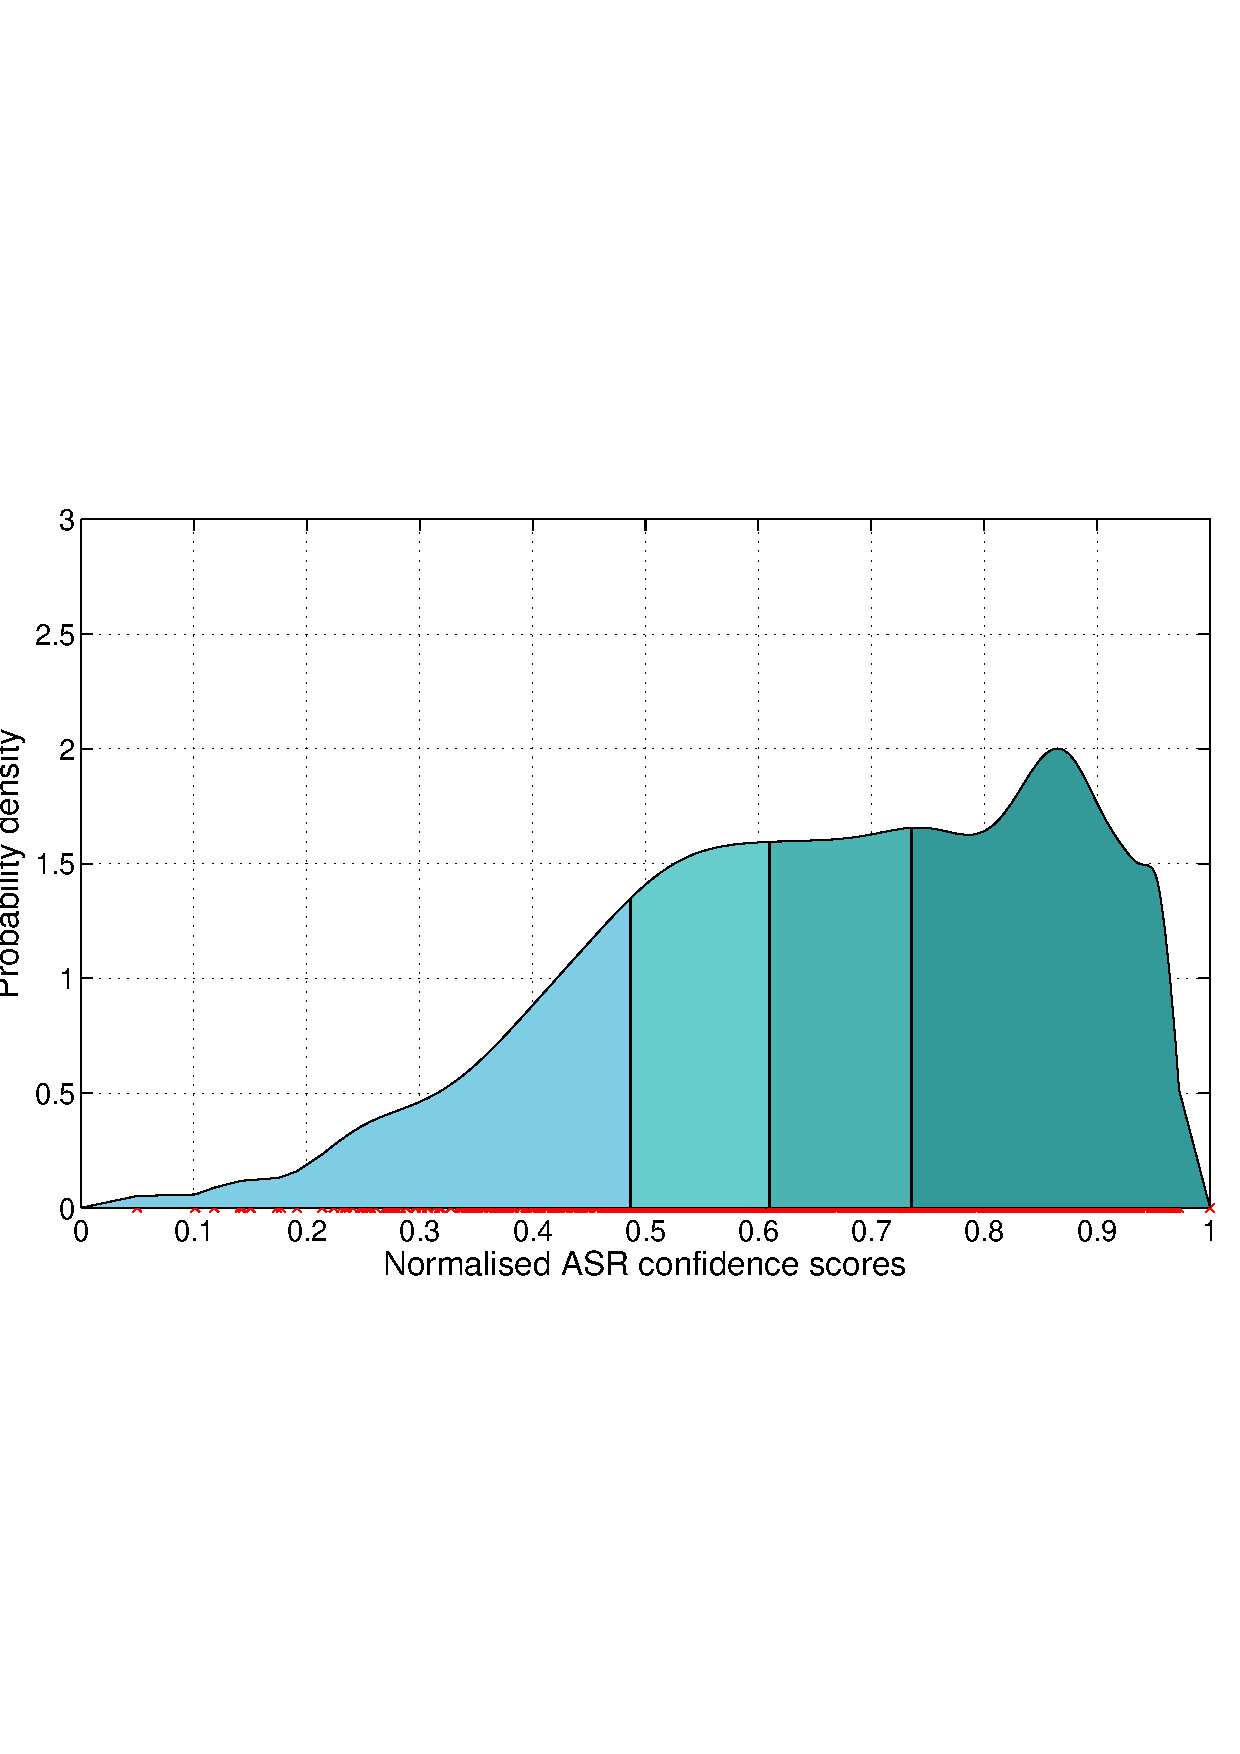
\includegraphics[scale=0.4]{imgs/asrconfidence.pdf} 
\caption{Probability density function for the probability values of the top hypothesis specified in the user dialogue act $a_u$, divided into four non-overlapping regions that respectively correspond to the first, second, third, and fourth+fifth quintiles of the distribution. Red crosses on the X axis represent the actual probability values used to construct the kernel density function. }
\label{fig:asrconfidence-exp3}
\end{figure}


\subsection{Approach 2: factored statistical model}
\label{sec:approach2}

The second approach developed for this experiment consists of a statistical model whose parameters are estimated from the Wizard-of-Oz data set collected for the experiment. We assume that both the transition model and utility model of the domain are initially unknown. 

Both this approach and Approach 3 assume that the domain can be captured with a planning horizon limited to the present time step.  In other words, the approach does not rely on online forward planning (which is often practically difficult to reconcile with real-time constraints) and directly selects the action yielding the highest utility in the current dialogue state.\footnote{In other words, the utility model represents what is called a $Q$-value model in reinforcement learning.} The approach stands relatively close to the POMDP-based systems described in Chapter \ref{chap:probmodelling}, with the notable difference that the estimation of model parameters is performed in this experiment on the basis of Wizard-of-Oz data rather than through a user simulator. 

\subsubsection*{Domain modelling}

Figure \ref{fig:unstructuredmodel-exp3} shows the factored model employed to structure the dialogue domain of the experiment.  As evidenced in the figure, the domain models are factored in four major distributions (the three first ones being part of the transition model, while the fourth one is a utility model): 
\begin{itemize}
\item The task completion model $P(\mathit{completed\mbox{-}task}\, | \, i_u, a_m)$ describes the probability that the current intention $i_u$ is fulfilled by the last system action $a_m$.  The task completion model $P(\mathit{completed\mbox{-}task}\, | \, i_u, a_m)$ is essentially a deterministic distribution that marks the task as completed when the executed action $a_m$ fulfils the user intention $i_u$,  and as not completed in other cases. %The task completion model is therefore defined without parameters. 
\item The user goal model $P(i_u' \, | \, i_u, \mathit{completed\mbox{-}task}, \mathit{perceived'}, \mathit{carried'})$ encodes the likelihood of a new user intention $i_u'$ given the current intention $i_u$, task completion $\mathit{completed\mbox{-}task}$, as well as the two contextual variables $\mathit{perceived}$ and $\mathit{carried}$. 
\item The user action model $P(a_u'\, | \, i_u', a_m)$ describes the probability of the next user dialogue act $a_u'$ given the user intention $i_u'$ and the last system action $a_m$.
\item Finally, the utility model $U(a_m', i_u', a_u', \mathit{carried'}, \mathit{perceived'}, \mathit{motion'})$ describes the utility of a given system action $a_m'$ given the user intention $i_u'$, last user dialogue act $a_u'$, robot motion status $\mathit{motion'}$ and contextual variables $\mathit{carried}$ and $\mathit{perceived}$. 
\end{itemize}

\begin{figure}[h]
\centering
\includegraphics[scale=0.4]{imgs/unstructuredmodel.pdf} 
\caption{Factored transition and utility models for the dialogue domain.}
\label{fig:unstructuredmodel-exp3}
\end{figure}

\subsubsection*{Dimensionality reduction}

% As shall be explained shortly, the probabilistic models developed in this approach do include a fair amount of internal structure and rely on a number of assumptions to limit the number of parameters, but without resorting to the more advanced modelling techniques that characterise rule-structured models (such as latent rule nodes and quantification). The purpose of this model is thus to evaluate the performance of a classical statistical approach when provided with the Wizard-of-Oz interaction data set at our disposal. 

The four factored models remain however too large to be directly estimated from the limited amounts of data made available from the Wizard-of-Oz interactions.  We therefore introduced a range of additional constraints and simplifying assumptions that aim to further reduce the number of parameters associated with the model.

%\begin{align}
%&&&P(\mathit{completed\mbox{-}task}\!=\!\mathit{true} \, | \, i_u, a_m) = \nonumber \\
%&&& \ \ \ \ \ \ \ \ \ \ \ \ \ \ \ \ \ \ \ \  \begin{cases} 1 & \text{if } \ a_m \  %\text{fulfills the intention } i_u \\
%0 & \text{if } \ a_m\!=\!\mathrm{AskRepeat} \text{ or } \mathrm{AskConfirm} \\
%\theta_{\text{changeOfMind}} & \text{otherwise} \end{cases} \label{eq:completedtask-exp3}
%\end{align} 

The first simplifying assumption pertains to the user goal model $P(i_u' \, | \, i_u, \mathit{completed\mbox{-}task},$ $\mathit{perceived}, \mathit{carried})$, and rests on the idea that the user intention remains more or less constant -- modulo a small probability of revision to account for sudden changes of mind on the part of the user -- until the task is marked as completed. The values of the two contextual variables $\mathit{perceived}$ and $\mathit{carried}$ variables are furthermore grouped into two partitions: empty set or non-empty set. These two simplifications reduce the number of parameters required for the model to four Dirichlet distributions, each with 18 dimensions (which is the number of possible user intentions). 

%\begin{align}
%&&&P(i_u'  = x \, | \, i_u, \mathit{completed\mbox{-}task}, \mathit{perceived}, \mathit{carried}) = \nonumber \\
%&&& \ \ \ \ \ \ \ \ \ \ \ \ \ \ \ \ \ \ \ \  \begin{cases} \theta_{i_u'\!=\!x|\mathit{perceived}, \mathit{carried}} & \text{if } \  \mathit{completed\mbox{-}task}= true \\
%\mathbf{1}(x = i_u) & \text{otherwise} \end{cases}
%\end{align}

We also compressed the size of the user action model $P(a_u'\, | \, i_u', a_m)$ by exploiting the fact that only a fraction of user dialogue acts $a_u'$ are locally relevant for a given user intention $i_u'$ and last system action $a_m$.  A manually specified function $relevant: \mathit{Val}(i_u) \times \mathit{Val}(a_m) \rightarrow 2^{\mathit{Val}(a_u)}$ is used to derive the set of relevant user actions given a particular pair of user intention and system action. For instance, the relevant dialogue acts for the user intention $\mathrm{Move(Left,Short)}$ are $\mathrm{Ask(Move(Left,Short))}$, $\mathrm{RepeatLast}$, $\mathrm{Confirm}$, $\mathrm{Disconfirm}$, $\mathrm{Stop}$ and $\mathrm{Grounding}$. The resulting set of parameters associated with the user action model contains 133 Dirichlet distributions, each with 6 dimensions (the number of relevant actions allowed per intention). 

The third and final heuristic is to reduce the number of relevant system actions in the utility distribution $U(a_m', i_u', a_u', \mathit{carried}, \mathit{perceived}$, $\mathit{motion'})$.  Similarly to the user action model, one can exploit the fact that only a fraction of system actions are relevant in a given state, and that the non-relevant ones have a constant negative utility. In order to express this constraint, we first define a function $best: \mathit{Val}(i_u) \times \mathit{Val}(\mathit{perceived}) \times \mathit{carried} \rightarrow \mathit{Val}(a_m)$ that maps each user intention and context to the ``best'' action that can be executed at that state if we were to assume no uncertainty. This best action is identical to the action selected by the finite state automaton in Figure \ref{fig:fsa-exp3}. In addition to this best action, we also allow the actions $\mathrm{AskConfirm(i_u')}$, $\mathrm{AskRepeat}$ and $Do(Stop)$ to be executed at any state. The utility distribution is then expressed as: 
\begin{align}
&&& U(a_m', i_u', a_u', \mathit{carried}, \mathit{perceived}, \mathit{motion'}) = \nonumber \\
&&& \ \ \ \ \ \ \  \begin{cases} \ \theta_{\text{best}(i_u', \mathit{carried}, \mathit{perceived})} & \text{if } \ a_m = best(i_u', \mathit{carried}, \mathit{perceived}) \\ 
\ \theta_{\text{askConfirm}(i_u', \mathit{carried}, \mathit{perceived})} & \text{if } \ a_m = \mathrm{Confirm(i_u')} \\
\ \theta_{\text{askRepeat}(a_u, \mathit{motion'})} & \text{if } \ a_m = \mathrm{AskRepeat} \\
\ \theta_{\text{stop}(a_u,\mathit{motion'})} & \text{if } \ a_m = \mathrm{Stop} \\ 
\mbox{-}10 & \text{otherwise}
\end{cases} \label{eq:utilunstruct-exp3}
\end{align}

The factorisation of the utility model in Equation \eqref{eq:utilunstruct-exp3} results in 296 parameters. In total, the numbers of parameters associated with all factored models in this approach (including both univariate and multivariate parameters) equals to 433.

\subsubsection*{Parameter estimation}

The parameter estimation follows the Bayesian learning procedure presented in Chapter \ref{chap:wozlearning}. The learning algorithm operates by cycling through the Wizard-of-Oz training data and updating the parameter distributions after each data point using Bayesian inference.  The wizard is assumed to act rationally in most cases and select the action that yields the highest utility given the current dialogue state. 

It should be noted that, in contrast to the experiment presented in Section \ref{sec:wozlearning-experiments} (which concentrated on the estimation of a single model), the parameters to estimate in this setting include both the transition model and the utility model.  The learning algorithm is thus an instance of a joint optimisation problem, as the system must simultaneously optimise both models in order to find the parameters that provide the best fit for the Wizard-of-Oz dataset as a whole. 

The parameters of categorical distributions are all encoded by Dirichlet distributions initialised with weakly informative priors, while the utility parameters are encoded by uniform distributions with a support range of $[-10, 30]$.  Section \ref{sec:learningcurve-exp3} provides more details on the learning curve followed during the estimation process.
% as well as the degree of agreement between the learned model and the ``gold standard'' actions selected by the wizard. 

\subsection{Approach 3: rule-structured model}

The final dialogue management approach developed in this experiment is couched in the formalism of probabilistic rules presented in this thesis.  

%approach relies here on the specification of probabilistic rules to express these models, and the parameter of these rules are optimised on the basis of the Wizard-of-Oz data set.

\subsubsection*{Domain modelling}

The general structure of the domain remains similar to the one shown in Figure \ref{fig:unstructuredmodel-exp3}.  As in the second approach, the models are decomposed into a task completion model, a user goal model, a user action model, and a utility model.  Action selection is again formalised as a search for the highest-utility action in the current state (assuming a planning horizon limited to the current time step).  However, in contrast to Approach 2, the internal structure of the domain models is here encoded through probabilistic rules instead of standard categorical distributions:
\begin{itemize}
\item The task completion model $P(\mathit{completed\mbox{-}task}\, | \, i_u, a_m)$ is encoded by one single deterministic rule that define when the current intention $i_u$ is fulfilled by the system action $a_m$. 
\item The user goal model $P(i_u' \, | \, i_u, \mathit{completed\mbox{-}task}, \mathit{perceived'}, \mathit{carried'})$ consists of a collection of seven rules that define the probability of the new user intention $i_u'$ given the dialogue context. One rule defines the prior probability of the user intentions $\mathrm{Move(\mathit{x})}$, four rules specify the prior probability of $\mathrm{PickUp(\mathit{x})}$, $\mathrm{WhatDoYouSee}$ and $\mathrm{DoYouSee(\mathit{x})}$ (depending on the value of the $\mathit{perceived}$ variable), one rule specify the prior probability of $\mathrm{Release}$ (depending on the value of the $\mathit{carried}$ variable), and one final rule specifies the probability of the $\mathrm{Greeting}$ and $\mathrm{Closing}$ intentions (depending on the last system move). 

\item The user action model $P(a_u'\, | \, i_u', a_m)$ is formalised with two rules that maps user intentions to their potential verbal realisations in terms of user dialogue acts. The first rule expresses the likelihood of various user dialogue acts depending on the user intention and last system action (in particular, whether the system uttered a clarification or confirmation request).  The second rule expresses the likelihood of the $\mathrm{Ask(Stop)}$ and $\mathrm{Disconfirm}$ actions during the execution of a physical movement.

\item Finally, the utility model $U(a_m', i_u', a_u', \mathit{carried'}, \mathit{perceived'}, \mathit{motion'})$ is encoded with a total of eleven utility rules.  The model essentially contains one rule for each family of possible system actions.  There is therefore one rule to define the relative utility of movement actions, one rule for grasping actions, one rule for the release action, two rules for the $\mathrm{Describe(\mathit{x})}$, $\mathrm{ConfirmDetection}$ and $\mathrm{DisconfirmDetection}$ actions, one rule to handle the  $\mathrm{Greet}$ and $\mathrm{Goodbye}$ actions, three rules for the clarification and confirmation requests, and one rule to stop the current movement. The last rule fixes an initial, negative utility for all actions to ensure that non-relevant actions have a utility lower than zero.  

\end{itemize}

The probability and utility models described by these rules include a total of 28 parameters, amongst which 15 probability parameters and 13 utility parameters.  The complete specification of the domain is provided in Appendix \ref{chap:domainspecs} (Section \ref{sec:domainspecs-usereval}). 

\subsubsection*{Parameter estimation}

The rule parameters were optimised on the basis of the collected Wizard-of-Oz data following the same procedure as the one followed for the second approach.  The parameters of probability rules are all encoded by Dirichlet distributions (of varying dimensions, from 2 to 10 depending on the rule) initialised with weakly informative priors, while the parameters of utility rules are encoded by uniform distributions on the support range $[-10, 30]$.  


\subsection{Learning curves}
\label{sec:learningcurve-exp3}

Figure \ref{fig:curve-exp3} presents the learning curves that characterise the three dialogue management approaches presented in the previous pages. The Wizard-of-Oz data set described in Section \ref{sec:wozcollection-exp3} was first divided into a training set of 9 interactions (summing up to 770 system turns) and a test set with one single interaction containing a total of 71 system turns. Based on this division, we measured the degree of agreement between the action selected by the system (on the basis of its model parameters) and the one selected by the wizard. This measurement is repeated at regular intervals during the parameter estimation process.  It should be stressed once more that system actions that do not correspond to the ones selected by the wizard are not necessarily wrong or inappropriate, as they may reflect different but perfectly legitimate conversational strategies. The degree of agreement between the model and the wizard examples is however a good indication of the model ability to capture the dynamics of the interaction as well as the trade-offs of the action selection process. 

\begin{figure}[h]
\vspace{3mm}\centering\includegraphics[scale=0.35]{imgs/curve-exp3.pdf}
\caption{Learning curve for the three dialogue management approaches on the Wizard-of-Oz data set.  The figure shows how the agreement between the best system action and the actual wizard action evolves as a function of the number of processed training samples.  The agreement is calculated on a separate test set of 71 system turns.}
\label{fig:curve-exp3}
\end{figure}


The learning curves in Figure \ref{fig:curve-exp3} illustrate the evolution of the degree of agreement as the function of the number of training samples processed by the learning algorithm.  As the finite-state approach is entirely handcrafted and does not include any parameters to optimise, its agreement with the wizard actions remains constant at all time steps. We can notice from the learning curves that both statistical approaches (Approach 2 and 3) do improve their agreement as they process more and more training samples, but do so at different learning speeds.  While the rule-structured model is able to converge to a high-quality dialogue policy after observing only a fraction of the training data, the traditional, factored statistical model converges at a slower rate due to its larger set of parameters and weaker generalisation capacity. 

The final agreement results obtained after processing the complete training set are shown in Table \ref{table:learning-exp3}.  As one can observe, the rule-structured approach is the one that is best able to imitate the conversational behaviour of the wizard. 

\begin{table}[h]
\begin{center}
\begin{tabular}{|l|c|} \hline
\textit{Type of model} & \textit{Agreement with the wizard actions (in \%) } \\ \hline \hline
Finite state automaton & 43.66 \\ \hline
Factored statistical model & 54.93 \\ \hline
Rule-structured model & \textbf{71.83} \\ \hline
\end{tabular}
\end{center}
\vspace{-2mm}
\caption{Agreement results on the test test for the three approaches.}
\vspace{-2mm}
\label{table:learning-exp3}
\end{table}

\section{User trials}

In order to assess the relative performance of the three dialogue management approaches presented in the previous section, we conducted a total of $3 \times 37$ user trials, which we now describe in detail. We start by exposing the experimental setup employed in the user trials, and then present and discuss the empirical results. 

\subsection{Experimental setup}

\subsubsection*{Participants}

The experiment was carried out with a total of 37 participants (16 males and 21 females).  The average age of the participants was 30.6 years (standard deviation: 7.8). The participants were recruited mainly amongst students and employees of the Department of Informatics at the University of Oslo. All participants were non-native speakers of English. To facilitate the recruitment of participants, a small monetary reward was offered to the participants upon the completion of the experiment. 

\subsubsection*{Preliminaries}

Before the start of each trial, we briefed the participants about the interaction scenario and the physical and conversational capabilities of the robot. To give the participants a better sense of what the robot can understand (and what falls outside the scope of the dialogue domain), we provided each participant with an instruction sheet detailing the different kinds of movements the robot can perform, as well as a few examples of verbal instructions for each.

Before the start of the experiment, the participants were asked to fill a short survey about their age, gender, and their expectations regarding the robot verbal behaviour. The user expectations were measured with a set of six multiple-answer questions as shown in Figure \ref{fig:expectations}. The questions cover multiple aspects that may affect the interaction quality in the domain, such as the comprehension abilities of the robot (Q1), its ability to find select appropriate reactions (Q2), its use of clarification requests (Q3), its ability to distinguish between noise and actual utterances (Q4 and Q5), and finally the naturalness of the interaction (Q6). One should note that the participants were told during the briefing phase to be aware of the technical limitations of the speech recogniser. The user responses must therefore be read in the light of this cautionary statement. 


The first and most evident purpose of this preliminary survey is to allow us to compare the prior expectations of the users with their actual experiences.  As shown by e.g.\ \cite{JokinenH06}, such comparison can yield interesting insights on the factors that empirically influence user satisfaction and their variability amongst different groups of users.  In addition, the survey also served as an indirect mean to direct the user attention towards the aspects of the robot behaviour that are of particular relevance for this study -- namely, the robot's choice of dialogue moves. 


\begin{figure}[h]
\begin{center}
\includegraphics[scale=0.5]{imgs/expectations.pdf}
\end{center} 
\caption{Prior user expectations about the robot conversational abilities.}
\label{fig:expectations}
\end{figure}

\subsubsection*{User trials}

After filling the survey, each participant was requested to carry out three distinct dialogues (one for each dialogue management approach).  The order in which the three approaches were tested was shuffled before each trial to mitigate the effects of the ordering sequence on the results.\footnote{The interactions become indeed increasingly efficient as the user gets more accustomed to the robot and the task to perform.  The average duration of the first dialogue amounts to 6'31, while the average duration of the second dialogue is reduced to 5'08, and the duration of the last dialogue goes down even further to 4'40.}  The participants did not have a time limit to complete the task. Immediately after each dialogue, the participants were asked to fill a small survey to determine how they subjectively perceived the interaction.  The survey was once more divided into six multiple-answer questions (cf. below).  

All interactions were captured on video, totalling about 12 hours of footage. In addition to the videos, the dialogue system also logged all user and system turns occurring in the interaction along with their associated dialogue state.


\subsection{Results}
\label{sec:results-exp3}

\subsubsection*{Objective metrics}

In line with previous work on the evaluation of spoken dialogue systems \citep[see e.g.][ch. 6 for an overview]{2009Jokinen}, we defined a set of metrics aimed at measuring the quality and efficiency of the recorded dialogues.  The defined metrics and their empirical values for three approaches are shown in Figure \ref{fig:objective}.

Although many evaluation schemes also include explicit measures of task completion in their metrics, we found such measure to be difficult to incorporate in our experimental setup, as the participants did not really have the possibility to end a task before its conclusion. Some dialogues had to be terminated before the full completion of the task but these cases were due to external causes such as hardware failures (e.g.\ system crash or physical collapse of the robot).
 
The metrics were calculated on the basis of the interaction logs produced by the dialogue system during the course of the dialogue. As the interaction logs are generated automatically, the counts of user turns correspond to the number of speech recognition results and do not necessarily correspond to the actual user turns in the dialogue (due to spurious results caused by ambient noise). We can observe from Figure \ref{fig:objective} that the rule-structured model produces on average shorter and more efficient dialogues than the two baselines.  In particular, on the basis on its parameter estimation on the Wizard-of-Oz training set, the rule-structured model systematically assigned higher utilities to confirmation requests (\utt{should I do X?}) in comparison to repetition requests (\utt{Sorry, could you repeat?}) and 
consequently never asked the user to repeat the last utterance. The number of system turns is also notably shorter than for the finite-state and factored statistical model, reflecting the fact that the rule-structured model is better able to filter out spurious recognition results. 

\begin{figure}[p]
\begin{center}
\includegraphics[scale=0.5]{imgs/objective.pdf}
\end{center} 
\caption{Objective metrics extracted from the collected dialogues. }
\label{fig:objective}
\end{figure}


\subsubsection*{Subjective metrics}

The subjective metrics reflect the answers to the six multiple-answer questions specified in the user survey. Each question allows for five alternative answers scale ranked from worst to best.  The six questions and the responses they received from the participants are shown in Figure \ref{fig:subjective}. As one can observe, the responses to the survey do seem to indicate that the rule-structured model was perceived to result in more effective and natural conversational behaviours. 


%\begin{enumerate}
%\item Did you feel that the robot correctly understood what you said?	\\
%\begin{footnotesize}\textit{Answers}: (1) Not at all \hspace{2mm} (2) Not very often \hspace{2mm}  (3) Half the time \hspace{2mm} (4) Most of the time \hspace{2mm} (5) Nearly always\end{footnotesize}

%\item Did you feel that the robot reacted appropriately to your instructions?	\\
%\begin{footnotesize}\textit{Answers}: (1) Not at all \hspace{2mm} (2) Not very often \hspace{2mm} (3) Half the time \hspace{2mm} (4) Most of the time \hspace{2mm} (5) Nearly always\end{footnotesize}

%\item Did you feel that the robot asked you to repeat or confirm your instructions ...\\	
%\begin{footnotesize}\textit{Answers}: (1) Very often \hspace{2mm} (2) Quite often \hspace{2mm} (3) Occasionally \hspace{2mm} (4) Rarely \hspace{2mm} (5) Never\end{footnotesize}

%\item Did you feel that the robot sometimes ignored when you were speaking?	\\
%\begin{footnotesize}\textit{Answers}: (1) Very often \hspace{2mm} (2) Quite often \hspace{2mm} (3) Occasionally \hspace{2mm} (4) Rarely \hspace{2mm} (5) Never\end{footnotesize}

%\item Did you feel that the robot sometimes thought you were talking when you were not?	\\
%\begin{footnotesize}\textit{Answers}: (1) Very often \hspace{2mm} (2) Quite often \hspace{2mm} (3) Occasionally \hspace{2mm} (4) Rarely \hspace{2mm} (5) Never\end{footnotesize}

%\begin{footnotesize}\item Did you feel that the interaction with the robot flowed in a pleasant and natural manner? \\
%\textit{Answers}: (1) Not at all \hspace{2mm} (2) Not very much \hspace{2mm} (3) More or less \hspace{2mm} (4) For the most part \hspace{2mm} (5) Definitely\end{footnotesize}
%\end{enumerate}


\begin{figure}[p]
\begin{center}
\includegraphics[scale=0.5]{imgs/subjective.pdf}
\end{center} 
\caption{Survey responses obtained from the participants in the user trial after each interaction. }
\label{fig:subjective}
\end{figure}

\subsubsection*{Summary of results}

Table \ref{table:results_exp3} summarises the results of both objective and subjective metrics and specifies the statistical significance of each observed difference between measures.  The results from the subjective metrics are calculated by mapping the qualitative answers to a scale from 1 to 5 (1 corresponding to the worst behaviour and 5 to the best) and averaging the results over all participants. 

In order to analyse the statistical significance of the results obtained for each metric, the table indicates the $p$-values for two distinct test statistics:\footnote{A $p$-value corresponds to the probability of obtaining a test statistic at least as extreme as the one actually observed if we presuppose that the null hypothesis is true.  We can therefore reject the null hypothesis whenever the derived $p$-value is lower than a certain significance level $\alpha$ (often set 0.05 or 0.01).}
\begin{itemize}
\item The first $p$-value is derived via the ANOVA procedure (Analysis of Variance) with one single factor corresponding to the chosen dialogue manager. The null hypothesis $H_0$ corresponds in this case to the assumption that the observed measures extracted with the three models are drawn from populations with the same mean values.  

\item As we are more specifically interested in the difference between the rule-structured approach and the two baselines, we also calculated a second test statistic that compares for each metric the means of the best and second-best approaches. The test statistic is in this case derived using Student's paired $t$-tests.

\end{itemize}

Results for which a statistically significant difference (with $\alpha = 0.05$) is found are decorated with a star sign. As one can observe from the table, 9 of the 15 metrics demonstrate statistically significant differences for the rule-structured model, while 4 metrics show higher means for the rule-structured model but without achieving statistical significance, and 2 metrics yield better results for the finite-state approach, although both without statistical significance. 

It is also useful to contrast the results obtained from the survey with the initial user expectations, as shown in Table \ref{table:compexpectation-exp3}.  We can observe that for all six questions, the actual system behaviour of the rule-structure approach exceeded the initial expectations of the user. 

\renewcommand{\arraystretch}{1.2}

\begin{sidewaystable}
\begin{tabular}{|cp{110mm}c|r:r:r|p{16mm}|p{16mm}|} \hline
&\centering \multirow{2}{*}{Metrics} & & \multicolumn{3}{c|}{Approaches} & \multirow{2}{*}{\parbox{16mm}{$\phantom{0000000}$ $p$-values ANOVA }} & \multirow{2}{*}{\parbox{16mm}{$\phantom{0000000}$ $p$-values $1^{\text{st}}$ vs. $2^{\text{nd}}$ ($t$-test) }} \\ \cline{4-6} 
&&& \multicolumn{1}{p{13mm}:}{\centering\begin{footnotesize}Finite-state automata\end{footnotesize}} & \multicolumn{1}{p{13mm}:}{\centering\begin{footnotesize}Factored statistical model\end{footnotesize}} & \multicolumn{1}{p{13mm}|}{\centering\begin{footnotesize}Rule-structured model\end{footnotesize}} & & \\ \hline \hline
& \vspace{-2mm} \textbf{Objective metrics}:  && & & & & \\ 
1.& Average number of repetition requests per dialogue && 18.68 & 12.24 & \textbf{0}$^{\mathbf{*}}$ & $9\!\times\!10^{-19}$ & $1\!\times\!10^{-16}$ \\
2.& Average number of confirmation requests per dialogue &&9.16 & 10.32 & \textbf{5.78}$^{\mathbf{*}}$ & $1.7\!\times\!10^{-4}$& $0.001$ \\ 
3.& Average number of repeated instructions per dialogue && 3.73 &
7.97 & \textbf{2.78}$^{\phantom{*}}$ & $3.8\!\times\!10^{-9}$ & $0.18$ \\ 
4.& Average number of ``$\mathrm{Disconfirm}$'' acts per dialogue &&\textbf{2.16} & 2.59 & 2.59$^{\phantom{*}}$ & $0.65$ & $0.33$ \\ 
5.& Average number of physical movements per dialogue & & \textbf{26.68}
 & 29.89 & 27.08$^{\phantom{*}}$ & $0.13$ &  0.80 \\ 
6.& Average number of (user and system) turns between movements &&3.63 & 3.10 & \textbf{2.54}$^{\mathbf{*}}$ & $4.\!\times\!10^{-4}$ & $2.2\!\times\!10^{-4}$ \\ 
7.& Average number of user turns per dialogue && 78.95 & 77.30 & \textbf{69.14}$^{\phantom{*}}$ & 0.17 & 0.11 \\ 
8.& Average number of system turns per dialogue && 57.27 & 54.59 & \textbf{35.11}$^{\mathbf{*}}$ & $4.4\!\times\!10^{-9}$ &  $5.6\!\times\!10^{-8}$\\ 
9.& Average duration of each dialogue  (in minutes) \vspace{3mm} && 6'18 & 7'13 &\textbf{ 5'24}$^{\mathbf{*}}$ & $1.4\!\times\!10^{-4}$ & 0.02 \\ \hdashline
& \vspace{-2mm} \textbf{Subjective metrics}:  && & & & & \\ 
&\textit{``Did you feel that ...}  && & & & & \\ 
10.&\ \ \textit{... the robot correctly understood what you said?''}  && 3.32 & 2.92 &  \textbf{3.68}$^{\mathbf{*}}$ & $1.3\!\times\!10^{-4}$ & 0.03 \\
11.& \ \ \textit{.. the robot reacted appropriately to your instructions?''}   && 3.70 & 3.32 & \textbf{3.86}$^{\phantom{*}}$ & $7.6\!\times\!10^{-3}$ & 0.23 \\
12.&\ \ \textit{... the robot asked you to repeat or confirm your instructions ...''}   & & 2.16 & 2.19 & \textbf{3.30}$^{\mathbf{*}}$ & $1.7\!\times\!10^{-9}$ & $4.7\!\times\!10^{-7}$ \\
13.&\ \ \textit{... the robot sometimes ignored when you were speaking?''}  & & 3.24 & 2.76 & \textbf{3.43}$^{\phantom{*}}$ & $6.7\!\times\!10^{-3}$ & 0.21 \\
14.&\ \ \textit{... the robot sometimes thought you were talking when you were not?''}  & & 3.43 & 3.14 & \textbf{4.41}$^{\mathbf{*}}$ & $3.4\!\times\!10^{-6}$ & $4.7\!\times\!10^{-5}$ \\
15.&\ \ \textit{... the interaction flowed in a pleasant and natural manner?''} \vspace{3mm}  & & 2.97 & 2.46 & \textbf{3.32}$^{\mathbf{*}}$ & $8.6\!\times\!10^{-4}$ & 0.03 \\ \hline
\end{tabular} \vspace{3mm}
\label{table:results_exp3}
\caption{Empirical results obtained for the user evaluation with a total of 37 participants, based on a set of 15 metrics (9 objective and 6 subjective). The $\mathbf{*}$ symbol indicates results that outperform the two other approaches with a level of statistical significance $\alpha = 0.05$. }
\end{sidewaystable}

\begin{table}[h]
\begin{center}
\begin{tabular}{|cp{55mm}c|r:r|p{18mm}|p{0mm}} \cline{1-6}
&\centering $\phantom{00000}$ Survey questions: $\phantom{00000}$ \textit{``Did you feel that ...} & & \multicolumn{1}{p{20mm}:}{\centering Initial expectations} & \multicolumn{1}{p{26mm}|}{\centering Rule-structured model} &\centering $p$-values ($t$-test) & \\ \cline{1-6} 
\rule{0pt}{4ex}    & \ \ \textit{... the robot correctly understood what you said?''}  &&  3.22 &  \textbf{3.68}$^{\mathbf{*}}$ &   0.025  & \\
& \ \ \textit{.. the robot reacted appropriately to your instructions?''}   && 3.35 & \textbf{3.86}$^{\mathbf{*}}$ & 0.004 & \\
&\ \ \textit{... the robot asked you to repeat or confirm your instructions ...''}   & & 2.68 & \textbf{3.30}$^{\mathbf{*}}$ & $4.6 \times 10^{-4}$ &  \\
&\ \ \textit{... the robot sometimes ignored when you were speaking?''}  &  & 2.89 & \textbf{3.43}$^{\mathbf{*}}$ & 0.015 & \\
&\ \ \textit{... the robot sometimes thought you were talking when you were not?''}  & & 3.81 & \textbf{4.41}$^{\mathbf{*}}$ &  0.001 & \\
&\ \ \textit{... the interaction flowed in a pleasant and natural manner?''} \vspace{1mm}  & & 2.92 &  \textbf{3.32}$^{\mathbf{*}}$ & 0.041 &  \\ \cline{1-6}
\end{tabular} 
\end{center}
\label{table:compexpectation-exp3}
\caption{Comparison between the initial expectations and the actual performance of the rule-structured approach . The $\mathbf{*}$ symbol indicates better-than-expected performance with $\alpha = 0.05$.\vspace{4mm} }
\end{table}

\subsection{Discussion}

\subsubsection*{Error analysis}

The empirical results derived from the user trials demonstrate the benefits of a hybrid modelling framework based on probabilistic rules compared to traditional approaches. Through a follow-up error analysis, we found this difference to be imputable to several factors, which we now describe.

Although the finite-state automaton functioned well in most trials, it often required multiple repetitions in order to reach sufficient confidence regarding the instruction to perform.  In comparison, the rule-structured model was able to accumulate evidence from several information sources (including the prior probabilities of the various instructions given the context) thanks to its explicit, probabilistic representation of the user intention $i_u$.  This possibility to accumulate evidence and exploit contextual knowledge enables the rule-structured model to zero in on the right instruction faster and more efficiently than the handcrafted model. One can observe this difference in the metrics 1 (number of repetition requests), 6 (number of turns per instructions) and 12 (frequency of clarification requests) of the user trial.  

Another interesting element we found in our analysis was that the factored statistical model operated well in the most common conversational situations, but was frequently led astray when encountering events that had not been observed in the Wizard-of-Oz training set. In particular, although the user action model $P(a_u'\, | \, i_u', a_m)$ offered reasonable estimates for the most prevalent user intentions and dialogue acts, this was not the case for less common instructions which had few or no occurrences in the training set.  This disparity in the estimated distributions often resulted in the dialogue system getting stuck in unseen dialogue states and selecting suboptimal actions.  Although it was trained on the exact same data, the rule-structured approach did not suffer from this data sparsity in the same extent due to its more powerful generalisation abilities. This difference can be clearly noticed in the metrics 3 (number of repeated instructions), 9 (average duration), 10 (quality of the robot's understanding) and 11 (appropriateness of the robot's behaviour). 

The finite-state automaton and the factored statistical model also encountered difficulties in filtering out spurious speech recognition hypotheses, especially the ones produced by the robot's own noise when executing physical movements.  This often led the robot to request the user to repeat an instruction when no instruction was actually uttered.  The rule-structured model proved to be better at filtering out these unwanted results.\footnote{The finite-state automaton employs a slightly higher threshold for moving from state $s_1$ to $s_3$ whenever the variable $\mathit{motion}$ is set to true. Although this mechanism did help in reducing the number of spurious results, it remained insufficient to fully distinguish between actual user utterances and erroneous recognitions.}  The metrics 8 (number of system turns) and 14 (ability of the robot to distinguish noise from speech) illustrate this discrepancy. 

Finally, it worth noting that the rule-structured model systematically assigned higher utilities to confirmation requests (\utt{should I do X?}) than repetition requests (\utt{sorry, could you repeat?}) when faced with unclear user instructions, as evidenced by the metric 1. While this characteristic of the learned rule-structured model initially came as a surprise (since the wizard did use some repetition requests in the Wizard-of-Oz interactions, although admittedly much less than confirmations), it proved to be an excellent conversational strategy for the domain, as participants perceived these confirmation requests to be much more natural and informative than repetitions. By contrast, the two baseline approaches relied much more heavily on repetition requests to elicit the user instructions.

\subsubsection*{Interpretation of the results}

The empirical results obtained from the user trials demonstrate that the hybrid modelling framework presented in this thesis is a viable and competitive alternative to classical dialogue management approaches.  The results are however subject to two caveats that should be mentioned.  Most importantly, it must be stressed that the results obtained for the two baselines are contingent on the particular design choices described in Section \ref{sec:approach1} and \ref{sec:approach2}.  Although these design choices are in our view relatively uncontroversial and do follow standard practices in the field of dialogue management, there is no doubt that these approaches could be further improved through more elaborate optimisation methods and parameter tuning. The intended purpose of the user evaluation was however \textit{not} to compare probabilistic rules with the ``best possible'' handcrafted and statistical techniques, as such characterisation would make little sense and remain impossible to prove in practice. Instead, the empirical results presented in the previous pages are best interpreted as a comparison between approaches featuring the same level of sophistication in their representation of the dialogue domain, but differing with one another along two dimensions:
\begin{itemize}
\item The finite-state automaton and the rule-structured model share the same domain knowledge and mappings between user instructions and corresponding system actions.  They however diverge in their account of uncertainty: while the automaton relies on confidence thresholds, the rule-structured model employs probabilistic reasoning to infer the most likely instruction given the observed inputs, prior likelihoods and external context.
\item Analogously, the factored statistical model and the rule-structured model share the same conditional dependencies between variables, domain-specific constraints, and training data. They however differ in the amount of internal domain structure introduced into the probabilistic model, and therefore in the numbers of corresponding parameters to estimate.
\end{itemize}

Furthermore, we must also highlight the fact that the results were obtained in a context of a dialogue domain that simultaneously exhibits (1) high levels of noise and uncertainty, (2) a relatively complex relational structure and (3) small amounts of available training data.  Although these three characteristics are common to many  dialogue domains, one should be wary of extrapolating these results to domains that do not share these properties.  For instance, dialogue domains in which most state variables are fully observed might be better addressed by purely symbolic techniques instead of relying on a hybrid approach. Similarly, dialogue domains that can draw on large amounts of training data might not have a direct need for the kind of expert domain knowledge incorporated in probabilistic rules.   In our experience, such cases constitute however the exception rather than the rule: most dialogue domains \textit{do} have substantial levels of uncertainty to confront, a rich internal structure, and only limited in-domain dialogue data (if any at all).


\section{Conclusion}

This chapter presented an extensive user evaluation of the hybrid dialogue modelling framework developed in this thesis.  The experiment was designed to compare a dialogue manager relying on probabilistic rules against two baselines that respectively correspond to a purely handcrafted dialogue manager (expressed as a finite-state automaton) and a purely statistical dialogue manager (based on factored models). 

The experiment was again set in a human--robot interaction domain.  The participants were asked to instruct the robot to locate a given object, pick it up and bring it back to the starting position.  Each of the 37 participants performed 3 dialogues (one for each dialogue management approach), thus amounting to $3 \times 37$ collected interactions.  After each interaction, the participants completed a survey with 6 questions inquiring about their perception of the dialogue.  

The three approaches were compared on the basis of 15 metrics with the aim to measure the quality and efficiency of the dialogues. The 15 metrics included both the user answers to the survey questions as well as 9 objective metrics extracted from the interaction logs.   The empirical results indicate that the rule-structured approach outperforms the two baselines on both objective and subjective metrics, with statistically significant differences for 9 metrics. The outcome of this user evaluation provides as a consequence further empirical support for the central argument developed in this thesis, namely that the formalism of probabilistic rules is well-suited to capture the structure of dialogue domains and can contribute to the development of more robust and conversationally competent dialogue systems through a combination of expert domain knowledge and probabilistic reasoning. 


% note about our approach: generalisation enable a better account of the data sparsity problem.  plus, the state dynamics are not lost since we perform belief update.  Finally, the appraoch can be seen as an initial boostrapping that can then be further refined through online reinforcement learning (Bayesian prior), as in Williams etc. also, we learn utilities, not a direct classification. Also: a user simulator is difficult for situated and open-ended environments.  we learn a POMDP policy by simulation
